\documentclass{aa}%\IEEEoverridecommandlockouts
% The preceding line is only needed to identify funding in the first footnote. If that is unneeded, please comment it out.
\usepackage{cite}
\usepackage{amsmath,amssymb,amsfonts}
\usepackage{algorithmic}
\usepackage{graphicx}
\usepackage{textcomp}
\usepackage{xcolor}
\usepackage{physics}
\usepackage{tikz}

\newcommand{\C}{\mathbb{C}}
\newcommand{\Cn}{\mathbb{C}^n}
\newcommand{\R}{\mathbb{R}}
\newcommand{\Rn}{\mathbb{R}^n}
\newcommand{\Hilbert}{\mathcal{H}}
\newcommand{\ci}{\dot{\imath}}
\newcommand{\stdbase}{\left\langle \textbf{e}_k \right\rangle_{1\leq k\leq n}}
\newcommand{\stdbaseelem}[1]{\left\langle \textbf{e}_{#1} \right\rangle}

\newcommand*\ieval[3]{\left.#1\right\rvert_{#2}^{#3}}
\newcommand*\ievalsimple[1]{#1 \Big|_{#1_a}^{#1_b}}

\newcommand{\centered}[1]{\begin{tabular}{l} #1 \end{tabular}}

\newcommand{\parentheses}[1]{\left( #1 \right)}

\begin{document}


\title{Numerical Solution of a Wave Function with Python*}

\subtitle{For Discrete Distribution Probability Spatial Sections}

\author{Avila Torres Miguel Angel
	\inst{1}
	%          \and
	%          C. Ptolemy\inst{2}\fnmsep\thanks{Just to show the usage
	%          of the elements in the author field}
}

\institute{Saint Thomas Aquinas University, Systems Engineering Faculty,\\
	Campus Avenida Universitaria - Edificio Santo Domingo de Guzmán: Av. Universitaria No. 45 - 202. Tunja - Boyacá\\
	\email{miguel.avilat@usantoto.edu.co}
	%         \and
	%             University of Alexandria, Department of Geography, ...\\
	%             \email{c.ptolemy@hipparch.uheaven.space}
	%             \thanks{The university of heaven temporarily does not
	%                     accept e-mails}
}

\date{\today}

% \abstract{}{}{}{}{} 
% 5 {} tokens are mandatory

\abstract
% context heading (optional)
% {} leave it empty if necessary  
{This paper describes how to solve the Schrodinger Equation given a valid wave function.}
% aims heading (mandatory)
{To }
% methods heading (mandatory)
{methods.}
{}
{}

\keywords{Wave function, Schrodinger Equation, Root finding, Integration, Interval, Limits}

\maketitle

\section{Introduction}

\section{Theoretical Framework}
\subsection{Wave Function}
The wave function of a state is commonly understood as its representation in a real vector space:
\begin{align}
	\Psi(\mathbf{r},t) &= \varphi(\mathbf{r})\psi(t)\\
	&= \braket{\varphi(\mathbf{r})}{\psi(t)}
\end{align}
where if $\ket{\Psi}$ is a vector of a Hilbert space then $\Psi(\mathbf{r})$ must be both normalizable and infinitely differentiable, with the requirement of $\braket{\Psi}{\Psi} = 1$ being true.\cite{wave}

\subsection{Probability of the wave function}
The wave function is interpreted as a probability distribution which must be equal to $1$. It is:
\begin{gather}
	\int\limits_{-\infty}^{\infty} | \Psi(\mathbf{r},t) |^2 d\textbf{r} = 1
\end{gather}
Where the integral is applied over $\mathbf{r}$ and it is done such that it express the position as such in spherical coordinates.\\

Observing this equation make us think about the probability for continuous statistical functions, which must be 1 for some range $ [a,b] $ (here $a=-\infty,b=\infty$). now, there also exists the measurement of the probability of finding a particle in some sector of the selected space, it is:
\begin{gather}
	\mathbf{P}_{\mathbf{a}_i \leq \mathbf{r}_i \leq \mathbf{b}_i}(t) = \int_{\mathbf{I}} | \Psi(\mathbf{r},t) |^2 d^n\mathbf{x};~~~\mathbf{r},\mathbf{I}\subset\mathcal{H}
\end{gather}
\subsection{Time-dependent general Schrödinger equation}
The Schrödinger equation is an equality which relates the state of a particle to its energy. The values for the energy which makes the equality relation hold are called eigenvalues of the wave function, the Schrödinger equation helps us to determine them when boundary conditions are given.\\

The time dependent general Schrödinger equation\cite{1} is
\begin{gather}
	i\hbar\frac{d}{dt}\ket{\Psi(t)} = \hat{H}\ket{\Psi(t)}
\end{gather}
Where the Hamiltonian operator $\hat{H}$\footnote{Note that the sum of potential and kinetic energy is the total energy in the system.} is:
\begin{align}
	\hat{H} &= \hat{T} + \hat{V}\\
	\hat{T} &= \frac{\mathbf{\hat{p}}\cdot\mathbf{\hat{p}}}{2m} = \frac{\hat{p}^2}{2m} = -\frac{\hbar^2}{2m}\nabla^2;~~~~~~\mathbf{\hat{p}}=-i\hbar\nabla\\
	\hat{V} &= V = V(\mathbf{r},t)
\end{align}
being $\hat{V}$ the potential energy, $\hat{T}$ the kinetic energy and $\mathbf{\hat{p}}$ the momentum operator. The equation can be written more completely as
\begin{gather}
	i\hbar\frac{d}{dt}\ket{\Psi(t)} = \left[ -\frac{\hbar^2}{2m}\nabla^2 + V(\mathbf{r},t) \right] \ket{\Psi(t)}
\end{gather}
Now, if the basis is relative to some point in the space we use\cite{2}
\begin{gather}
	i\hbar\frac{\partial}{\partial t}\Psi(\mathbf{r},t) = \left[\frac{-\hbar^2}{2m}\nabla^2 + V(\mathbf{r},t) \right] \Psi(\mathbf{r},t)
\end{gather}
where instead of a normal derivative we indicate that $\Psi$ depends on $\mathbf{r}$ (a position in the space) so that there is more meaning in the notation.\footnote{note that equation (5) is in terms of kets while (6) is in scalar terms.}\\

\subsection{Time-independent general Schrödinger equation}
In the case where time is not being considered, the Schrödinger equation has the form
\begin{align}
	\hat{H}\ket{\Psi} &= E\ket{\Psi}\\
	\left[ -\frac{\hbar^2}{2m}\nabla^2 + V(\mathbf{r}) \right] \ket{\Psi} &= E\ket{\Psi}
\end{align}
and is called time-independent Schrödinger equation; Here $E$ is the value of the total energy. Alternatively, the notation
\begin{align}
	\left[ -\frac{\hbar^2}{2m}\nabla^2 + V(\mathbf{r}) \right] \psi(\mathbf{r}) &= E\psi(\mathbf{r})
\end{align}
is also valid and does not represent any different meaning, the main difference is that $\psi$ sometimes is used for single particle systems\footnote{The equation relates some properties of a physical system, the wave function describes the expected position that the members of the system will have.} and $\Psi$ for multiple particle systems.\cite{3}\\

Finally, it is important to mention that given suitable conditions (typically $\Psi(\mathbf{r},0)$) the time independent Schrödinger equation determines $\Psi(\mathbf{r},t)$ for all value of $t$.\cite{grif}

\subsection{Hydrogen atom electron's wave function}
The possible wave functions of an electron in a Hydrogen atom are expressed in terms of spherical harmonics and generalized Laguerre polynomials. Now, it is convenient to use spherical coordinates, so that the wave function can be separated into functions of each coordinate \cite{hydro}
\begin{align}
	\psi(r,\theta,\phi) &= R(r)Y_{\ell}^m(\theta,\phi)\\
	&= \sqrt{\left( \frac{2}{na_0^*} \right)^3 \frac{(n-\ell-1)!}{2n[(n+\ell)!]}} e^{-r/ma_0^*} \left( \frac{2r}{na_0^*} \right)^\ell\\
	&~~~~~\cdot L_{n-\ell-1}^{2\ell+1}\left( \frac{2r}{na_0^*} \right) \cdot Y_\ell^m(\theta,\phi) 
\end{align}
this function is expressed in terms of other analytic functions which are simultaneously composed of some others as the spherical harmonic function:
\begin{align}
	Y_\ell^m(\theta,\phi) &= (-1)^m\sqrt{\frac{2\ell+1}{4\pi}\frac{(\ell-m)!}{(\ell+m)!}} P_{\ell m}(\cos(\theta))e^{im\phi}
\end{align}
the associated Legendre polynomial
\begin{align}
	L_n^{(\alpha)} &= \frac{x^{-\alpha}e^x}{n!} \frac{d^n}{dx^n}\left( e^{-x} x^{n+\alpha} \right)
\end{align}
and the Laguerre polynomial in the spherical harmonic
\begin{align}
	P_\ell^m(x) &= \frac{(-1)^m}{2^\ell \ell!}(1-x^2)^{m/2}\frac{d^{\ell+m}}{dx^{\ell+m}}(x^2-1)^\ell\\
	P_{\ell m}(x) &= (-1)^m \frac{(\ell-m)!}{(\ell+m)!}P_\ell^m(x)
\end{align}

The meaning of the wave function for the electron in an hydrogen atom is that: for the coordinates $r,\theta,\phi$, the quantum energy level $n = 1,2,3,4,\dots$, the quantum azimuthal number $\ell=0,1,2,3,...,(n-1)$ and the quantum magnetic number $m=-\ell,-\ell+1,-\ell+2,\dots,l$. $\psi$ is the probability of appearance for that electron at such given conditions and spatial point.

\subsection{Normalized hydrogen wave functions}
The following table shows the valid wave functions for the first three energy levels of an hydrogen atom
\begin{center}
	\def\arraystretch{2.5}
	\begin{tabular}{ccc|c|c}
		\hline
		\hline
		$n$ & $\ell$ & $m$ & $E_l$ & $\psi_{n\ell m}(r,\theta,\phi)$ \\
		\hline
		\hline
		1   & 0      & 0   & 1s & $\left( \sqrt{\pi}a_0^{3/2} \right)^{-1} e^{-r/a_0} $\\
		2   & 0      & 0   & 2s & $\left( 4\sqrt{2\pi}a_0^{3/2} \right)^{-1} \left[ 2 - \frac{r}{a_0} \right] e^{-r/2a_0}$\\
		2   & 1      & 0   & 2p & $\left( 4\sqrt{2\pi}a_0^{3/2} \right)^{-1} \frac{r}{a_0} e^{-r/2a_0} \cos(\theta)$\\
	 	\hline
		\hline
	\end{tabular}
\end{center}
Where $a_0 = \hbar^2/me^2 \approx 0.0529mn$.\cite{hydrofunctions}\footnote{It is the first Bohr Radius.}

\subsection{Monte Carlo integration method}
Monte Carlo integration is numerical integration method using random numbers, Monte Carlo integration has better accuracy than successively applied Simpson's Rule or the Trapezoidal method. The Monte Carlo numerical integral is defined taking as basis the integration of the following general function:
\begin{gather}
	I(f) = \int_{\Omega} f(\mathbf{\bar{x}}) d\mathbf{\bar{x}};~~~\Omega\subset\Rn
\end{gather}
where $\Omega$ is a region of $\Rn$. The value of the integral $I$ can be approximated by
\begin{align}
	V &= \int_{\Omega} d\mathbf{\bar{x}}\\
	I \approx Q_N \equiv V \frac{1}{N} \sum_{i=1}^{N}f(\mathbf{\bar{x}}_i) &= V\left\langle f \right\rangle;~~~\mathbf{\bar{x}}_i\in\Omega\\
	\lim\limits_{N\to\infty} Q_N &= I
\end{align}
which for $N$ tending to infinity is equal to the analytical integral due the law of large numbers. This numerical method has an estimated error formula of
\begin{align}
	\sigma_N^2 &= \frac{1}{N-1} \sum_{i=1}^{N} \left( f(\mathbf{\bar{x}}_i) - \left( \frac{1}{N} \sum_{i=1}^{N}f(\mathbf{\bar{x}}_i) \right) \right)\\
	&= \frac{1}{N-1} \sum_{i=1}^{N} \left( f(\mathbf{\bar{x}}) - \left\langle f \right\rangle \right)
\end{align}
which is the variance, and a standard deviation of
\begin{align}
	\sigma_N &= \left( \frac{1}{N-1} \sum_{i=1}^{N} \left( f(\mathbf{\bar{x}}) - \left\langle f \right\rangle \right) \right)^{1/2}
\end{align}

\section{Probability of the Hydrogen Wave Function in a Closed Spatial Section}
The Monte Carlo integration method applied over the general wave function of the hydrogen atom is
\begin{gather}
	I \approx \int_{\Omega} \xi(r_i,\theta_i,\phi_i) dr d\theta d\phi ~ \frac{1}{N} \sum_{i=1}^{N} \big|\psi_{n\ell m}(r_i,\theta_i,\phi_i)\big|^2
\end{gather}
where $\xi$ is the volume integral for an spatial volume section of a sphere. It is:
\begin{gather}
	\int_{\Omega} \xi(r_i,\theta_i,\phi_i) dr d\theta d\phi = \parentheses{ \parentheses{\int_{r_a}^{r_b} r dr}}
\end{gather}
where $\Omega$, by the Fubini's theorem the integral can be expressed as
\begin{gather}
	I \approx \int_{\phi_a}^{\phi_b}\int_{\theta_a}^{\theta_b}\int_{r_a}^{r_b} dr d\theta d\phi ~ \frac{1}{N} \sum_{i=1}^{N} \big|\psi_{n\ell m}(r_i,\theta_i,\phi_i)\big|^2
\end{gather}
being then
\begin{align}
	I &\approx \ievalsimple{r} \ievalsimple{\theta} \ievalsimple{\phi} ~ \frac{1}{N} \sum_{i=1}^{N} \big|\psi_{n\ell m}(r_i,\theta_i,\phi_i)\big|^2\\
	&\approx \Delta r~\Delta\theta~\Delta\phi ~ \frac{1}{N} \sum_{i=1}^{N} \big|\psi_{n\ell m}(r_i,\theta_i,\phi_i)\big|^2
\end{align}
the numerical integral, where
\begin{gather}
	\begin{array}{lll}
	\Delta r=r_b-r_a;&\Delta\theta=\theta_b-\theta_a;&\Delta\phi=\phi_b-\phi_a\\[10pt]
	r_i\in[r_a,r_b];&\theta_i\in[\theta_a,\theta_b];&\phi_i\in[\phi_a,\phi_b]	
	\end{array}
\end{gather}

\noindent Finally, as we would expect of a normalized wave function
\begin{gather}
	0 \leq I\left(\big|\psi_{n\ell m}(r_i,\theta_i,\phi_i)\big|^2\right) \to 1
\end{gather}
due the numerical error and that the integral of any squared normalized wave function is equal to one.

\subsection{Numerical solution for the first hydrogen's atom wave function}
Considering the first wave function
\begin{gather}
	\psi_{1,0,0}(r,\theta,\phi) = \left( \sqrt{\pi}a_0^{3/2} \right)^{-1} e^{-r/a_0}
\end{gather}
which cleverly shows how the probability of finding the electron in $1s$ decreases as the radial distance increases, and as $r=0$ reaches $\left( \sqrt{\pi}a_0^{3/2} \right)^{-1}$ being it its maximum value. ($r$ cannot be zero because it is a distance in spherical coordinates)\\

Its squared value is
\begin{gather}
	\abs{\psi_{1,0,0}(r,\theta,\phi)}^2 = \frac{1}{\pi a_0^3} e^{-2r/a_0}
\end{gather}
and represents the probability of finding the electron at a distance $r$ for any radial directions $\theta,\phi$\\

Replacing it on the previous derived formula we obtained, the finite numerical distribution probability of appearance for an electron in the hydrogen atom of electronic configuration $1s$ is
\begin{align}
	I &\approx \Delta r~\Delta\theta~\Delta\phi ~ \frac{1}{N} \sum_{i=1}^{N} \big|\psi_{n\ell m}(r_i,\theta_i,\phi_i)\big|^2\\
	\therefore I &\approx \Delta r~\Delta\theta~\Delta\phi ~ \frac{1}{N} \sum_{i=1}^{N} \left| \left( \sqrt{\pi}a_0^{3/2} \right)^{-1} e^{-r/a_0} \right|^2\\
	&\approx \Delta r~\Delta\theta~\Delta\phi ~ \frac{1}{N} \sum_{i=1}^{N} \frac{1}{\pi a_0^3} e^{-2r/a_0}
\end{align}

The following graph shows the wave function of H 1s
\begin{center}
	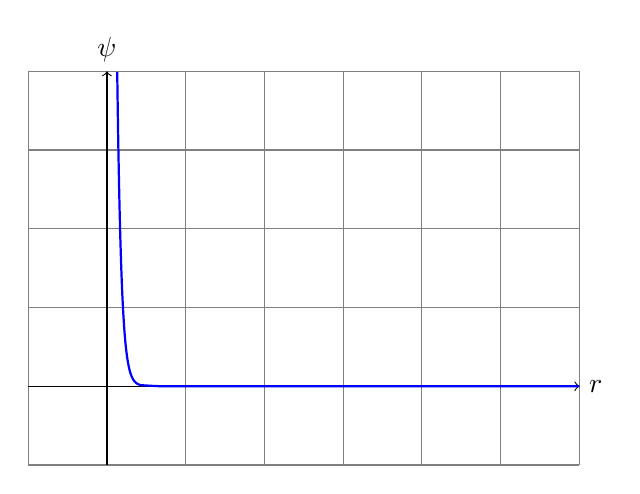
\begin{tikzpicture}
	\draw[step=1.0,gray,thin] (-1,-1) grid (6,4);
	\draw[->] (-1, 0) -- (6, 0) node[right] {$r$};
	\draw[->] (0, -1) -- (0, 4) node[above] {$\psi$};
	\draw[scale=1, thick, domain=0.13:0.44, smooth, variable=\x, blue] plot ({\x}, {e^(-\x/0.0529)/((3.141519)^(1/2) * (0.0529)^(3/2))});
	\draw[scale=1, thick, domain=0.43:6, smooth, variable=\x, blue] plot ({\x}, {e^(-\x/0.0529)/((3.141519)^(1/2) * (0.0529)^(3/2))});
	\end{tikzpicture}
\end{center}


\section{Conclusions}
\begin{itemize}
	\item 
	\item 
	\item 
	\item 
\end{itemize}

\newpage~\newpage
\begin{thebibliography}{00}
	\bibitem{wave} A. Lindner and D. Strauch, A Complete Course on Theoretical Physics. Springer, 2019.
	\bibitem{grif} D. Griffiths J. and D. Schroeter F., Introduction to Quantum Mechanics. Cambridge University Press, 2019.
	\bibitem{1} R. Shankar, ``Principles of Quantum Mechanics''. Springer, 2012.
	\bibitem{2}	``Schrodinger equation''\\
	http://hyperphysics.phy-astr.gsu.edu/hbase/quantum/Scheq.html\\
	(accessed: Sep. 20, 2020).
	\bibitem{3} ``In Quantum Mechanics is there any difference between $\psi$ and $\Psi$?''\\
	physics.stackexchange.com/questions/373993\\
	(accessed: Sep. 20, 2020).
	\bibitem{hydro} P. Tipler A. and G. Mosca, Physics for Scientists and Engineers. Macmillan, 2007.
	\bibitem{hydrofunctions} ``Hydrogen Wavefunctions'' http://hyperphysics.phy-astr.gsu.edu/hbase/quantum/hydwf.html (accessed: Sep. 22, 2020).
	\bibitem{montec} R. Cools and D. Nuyens, Monte Carlo and Quasi-Monte Carlo Methods. Springer, 2016. (1-46)
\end{thebibliography}

\end{document}
